\documentclass{article}

\usepackage[margin=1in]{geometry}
\usepackage{amsmath}
\usepackage{graphicx}
\usepackage{multicol}
\usepackage{fancyvrb}

\begin{document}
	
\title{ESOF 422 - Homework 2}
\author{Nathan Stouffer and Kevin Browder}

\maketitle
\newpage

\section*{Question 1}

	The class diagram for the Movie Rental system is displayed below in Figure \ref{fig:q1class}.
	\begin{figure}[h]
		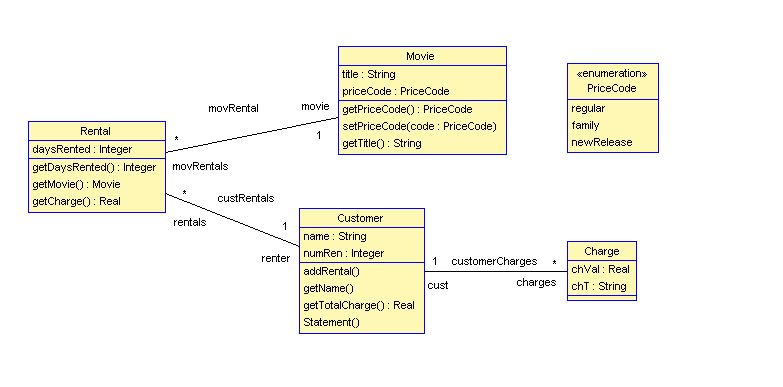
\includegraphics[width=\linewidth]{Q1Class.PNG}
		\caption{Movie Rental Class Diagram}
		\label{fig:q1class}
	\end{figure}
	
	\noindent
	Figure \ref{fig:q1class} generated with the following .use file:
\begin{Verbatim}
model MovieRental
enum PriceCode {regular, family, newRelease}

--classes

class Customer
attributes
	name:String
	numRen:Integer
operations
	addRental()
	begin
	end

getName()

getTotalCharge():Real
	begin
		declare totalCharge:Real, ch:Real;
		totalCharge:=0;
		for ren in self.rentals do
			ch:=ren.getCharge();
			totalCharge:=totalCharge + ch;
		end;
		result:=totalCharge;
	end;

Statement()
	begin
		declare aCharge:Charge, sm:Movie, ch:Real, t:String;
		self.numRen:=self.rentals->size();
		for ren in self.rentals do
			ch:=ren.getCharge();
			sm:=ren.getMovie();
			t:=sm.getTitle();
			aCharge:= new Charge;
			aCharge.chVal:=ch;
			aCharge.chT:=t;
			insert(self,aCharge) into customerCharges
		end
	end
end

class Rental
attributes
	daysRented:Integer

operations
	getDaysRented():Integer
		begin
			result := self.daysRented;
		end

getMovie(): Movie
	begin
		result := self.movie;
	end

getCharge():Real
	begin
		declare wrkCh:Real, m:Movie, pc:PriceCode,dy:Integer;
		m:=self.getMovie();
		dy:=self.getDaysRented();
		pc:=m.getPriceCode();

		wrkCh:=0;

		if pc=PriceCode::regular then
			wrkCh:=2.0;
			if dy > 2 then
				wrkCh:=wrkCh + (dy -2) * 1.5;
			end;
		end;

		if pc=PriceCode::family then
			wrkCh:=1.5;
			if dy > 3 then
				wrkCh:=wrkCh + (dy -3) * 1.5;
			end;
		end;

		if pc=PriceCode::newRelease then
			wrkCh:=dy * 3.0;
		end;

		result:=wrkCh;
	end
end

class Movie
attributes
	title:String
	priceCode:PriceCode
operations
	getPriceCode():PriceCode
		begin
			result := self.priceCode;
		end

setPriceCode(code:PriceCode)
	begin
		self.priceCode := code;
	end

getTitle():String
	begin
		result := self.title;
	end
end

class Charge
attributes
	chVal:Real
	chT: String
operations
end

--associations

--association between customer and rental
association custRentals between
	Customer [1] role renter
	Rental [0..*] role rentals
end

--association between rental and movie
association movRental between
	Rental [0..*] role movRentals
	Movie [1] role movie
end

--association between customer and charge
association customerCharges between
	Customer [1] role cust
	Charge [0..*] role charges
end

--constraints

constraints
context Customer
	inv maxRental:numRen <= 10
	inv agreement:rentals->size = numRen
	inv rentals:rentals->notEmpty
	inv daysRented:rentals->select(daysRented > 3)->notEmpty
\end{Verbatim}
	
	\noindent
	Using the code in the following .x file, we created the following object and sequence diagrams. Both of these were checked with our constraints.
	%TODO Kev, insert your .x file here. Then uncommment this block
\begin{Verbatim}
!create movie1:Movie
!create rental1:Rental
!create customer1:Customer
!create charge1:Charge

!insert (rental1, movie1) into movRental
!insert (customer1, rental1) into custRentals
!insert (customer1, charge1) into customerCharges

!set customer1.numRen := 1
!set rental1.daysRented := 4
\end{Verbatim}
	\newpage
	\noindent
	Figure \ref{fig:q1obj} shows the object diagram as well as the check on our invariants. Figure \ref{fig:q1seq} shows the sequence diagram.
	\begin{figure}[h]
		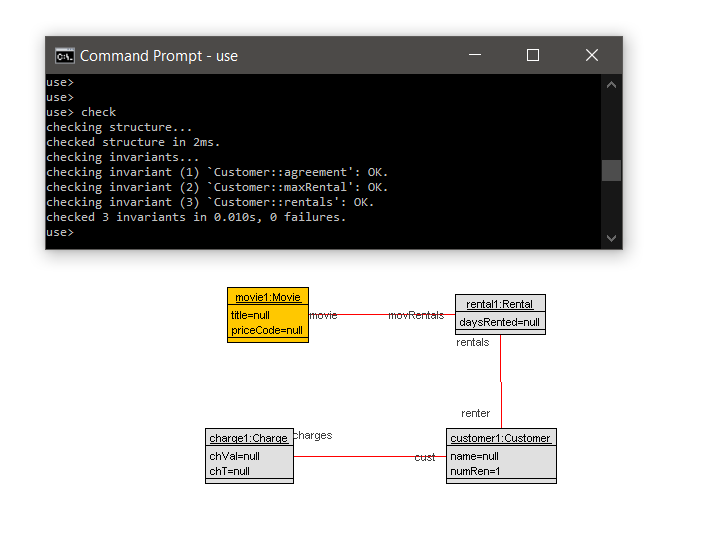
\includegraphics[width=\linewidth]{Q1ObjPNG.PNG}
		\caption{Object Diagram and Checking Constraints}
		\label{fig:q1obj}
	\end{figure}
	\newpage
	\begin{figure}[h]
		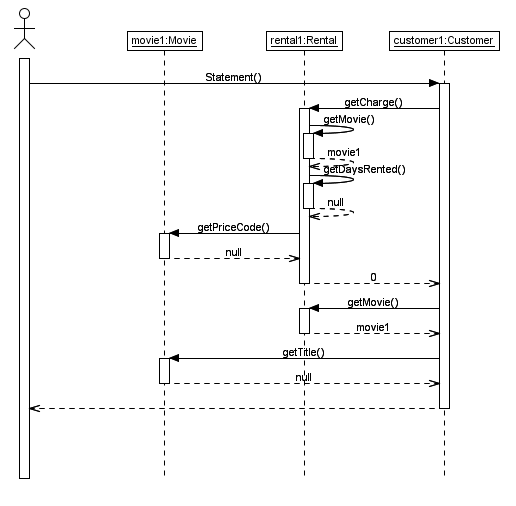
\includegraphics[width=\linewidth]{Q1Sequence.PNG}
		\caption{Sequence Diagram}
		\label{fig:q1seq}
	\end{figure}

	\noindent
	Note: On the assignment page, Question 2 had some questions that referrenced the model in Question 1. The invariants were included in the assignment file and we have included them in the .use file above.
	
	\newpage

\section*{Question 2}

	The class diagram for Royalty and Loyalty is displayed below in Figure \ref{fig:q2class}.
	\begin{figure}[h]
		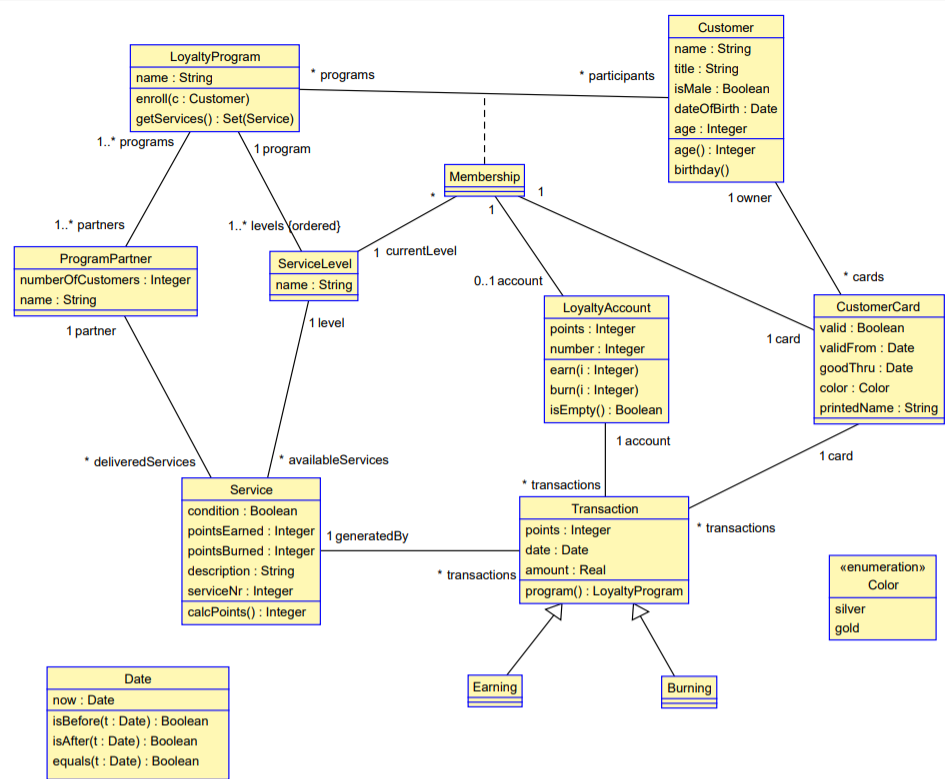
\includegraphics[width=\linewidth]{Q2Class.png}
		\caption{Royalty and Loyalty Class Diagram}
		\label{fig:q2class}
	\end{figure}
	
	\noindent
	The class diagram in Figure \ref{fig:q2class} was generated by the following .use file.
\begin{Verbatim}
-- Use file for question 2 of HW 2 in Adv. Software Engineering.
-- The file models a Loyalty Program system involving customers
-- that get services from Program Partners depending on their status

model LoyaltyProgram

-- enumerations

-- define enumeration for card type
enum Color {silver, gold}

-- classes

-- define Date class, this is a utility class
class Date
	attributes
		now : Date
	operations
		isBefore(t: Date): Boolean
		isAfter(t: Date): Boolean
	equals(t: Date): Boolean
end

-- define class LoyaltyProgram
class LoyaltyProgram
	attributes
		name: String
	operations
		enroll(c: Customer)
		getServices(): Set(Service)
end

-- define Customer class
class Customer
	attributes
		name: String
		title: String
		isMale: Boolean
		dateOfBirth: Date
		age: Integer 
	operations
		age(): Integer		-- derived
		birthday()
end

-- define ProgramPartner class
class ProgramPartner
	attributes
		numberOfCustomers: Integer
		name: String
	operations
end

-- define CustomerCard class
class CustomerCard
	attributes
		valid: Boolean
		validFrom: Date
		goodThru: Date
		color: Color
		printedName: String  -- derived
	operations
end

-- define LoyaltyAccount class
class LoyaltyAccount
	attributes
		points: Integer
		number: Integer
	operations
		earn(i: Integer)
		burn(i: Integer)
		isEmpty(): Boolean
end

-- define Service class
class Service
	attributes
		condition: Boolean
		pointsEarned: Integer
		pointsBurned: Integer
		description: String
		serviceNr: Integer
	operations
		calcPoints(): Integer
end

-- define Transaction class
class Transaction
	attributes
		points: Integer
		date: Date
		amount: Real
	operations
		program(): LoyaltyProgram
end

-- define class Burning
class Burning < Transaction
	attributes
	operations
end

-- define class Earning
class Earning < Transaction
	attributes
	operations
end

-- define Membership association class
associationclass Membership
	between
		LoyaltyProgram[0..*] role programs
		Customer[0..*] role participants
	attributes
	operations
end

-- define ServiceLevel class
class ServiceLevel
	attributes
		name: String
	operations
end

-- associations

-- association between LoyaltyProgram and ProgramPartner
association lp_pp between
	LoyaltyProgram[1..*] role programs
	ProgramPartner[1..*] role partners
end

-- association between LoyaltyProgram and ServiceLevel
association lp_sl between
	LoyaltyProgram[1] role program
	ServiceLevel[1..*] role levels ordered
end

-- association between Customer and CustomerCard
association c_cc between
	Customer[1] role owner
	CustomerCard[0..*] role cards
end

-- assocation between Membership and ServiceLevel
association m_sl between
	Membership[0..*]
	ServiceLevel[1] role currentLevel
end

-- association between Membership and LoyaltyAccount
association m_la between
	Membership[1]
	LoyaltyAccount[0..1] role account
end

-- association between Membership and CustomerCard
association m_cc between
	Membership[1]
	CustomerCard[1] role card
end

-- association between ProgramPartner and Service
association pp_s between
	ProgramPartner[1] role partner
	Service[0..*] role deliveredServices
end

-- association between Service and ServiceLevel
association s_sl between
	Service[0..*] role availableServices
	ServiceLevel[1] role level
end

-- association between Service and Transaction
association s_t between
	Service[1] role generatedBy
	Transaction[0..*] role transactions
end

-- association between LoyaltyAccount and Transaction
association la_t between
	LoyaltyAccount[1] role account
	Transaction[0..*] role transactions
end

-- association between CustomerCard and Transaction
association cc_t between
	CustomerCard[1] role card
	Transaction[0..*] role transactions
end

-- constraints

constraints

-- Question 1
-- context LoyaltyAccount::points
-- init: 0

-- context CustomerCard::valid
-- init: true

-- Question 2
context LoyaltyProgram
inv minLevels: levels->size() > 0

-- Question 3
-- context LoyaltyProgram::getServices():Set( Services)
-- body: partners->collect(deliveredServices)->asSet()

-- Question 4
-- context LoyaltyProgram::getServices(pp: ProgramPartner): Set(Services)
-- body: if partners->includes(pp)
--       then pp.deliveredServices->asSet()
--       else Set{}
--       endif

-- Question 5
-- from context of Service
context Service
inv serviceBurnGeqEarn: self.transactions->select(oclIsTypeOf(Earning))
		->forAll(t | pointsEarned > t.points)

-- from context of ProgramPartner
context ProgramPartner
inv: self.deliveredServices->forAll(ds | ds.transactions
		->select(oclIsTypeOf(Earning))->forAll(t | ds.pointsEarned > t.points))

-- Question 6
context LoyaltyProgram
inv noTransaction: self.partners->collect(deliveredServices)
		->forAll(ds | ds.pointsEarned = 0 and ds.pointsBurned = 0) 
		implies membership.account->isEmpty()

-- Question 7
context Customer::birthday()
pre birthdayPre: true
post birthdayPost: age = age@pre + 1
\end{Verbatim}
	
	\noindent
	Question 2 asks for a number of OCL statements. These statements are in the above .use file. However, we found that the use tool only allows for invariants and pre/post conditions. As such, we have commented out our answers for tasks that involve init and query operations. We then used the following .use file to generate an object diagram. \newline

\begin{Verbatim}
-- This file contains commands to create a possible state
-- of the Royalty and Loyalty model

-- create necessary objects
!create cust:Customer
!create prog:LoyaltyProgram
!create partner:ProgramPartner
!create slevel:ServiceLevel
!create account:LoyaltyAccount
!create card:CustomerCard

!create serv:Service
!set serv.pointsEarned := 1000

!create earn:Earning
!set earn.points := 900
!create burn:Burning
!set burn.points := 10

-- insert assocations
!insert (prog, cust) into Membership
!insert (prog, partner) into lp_pp
!insert (prog, slevel) into lp_sl

!insert (cust, card) into c_cc

!insert (Membership1, slevel) into m_sl
!insert (Membership1, account) into m_la
!insert (Membership1, card) into m_cc

!insert (partner, serv) into pp_s

!insert (account, earn) into la_t
!insert (account, burn) into la_t

!insert (serv, slevel) into s_sl
!insert (serv, earn) into s_t
!insert (serv, burn) into s_t

!insert (card, earn) into cc_t
!insert (card, burn) into cc_t
\end{Verbatim}
	
	\noindent
	The object diagram is displayed in Figure \ref{fig:q2obj}. Since there were no method calls, we chose not to disply a sequence diagram.
	
	\begin{figure}[h]
		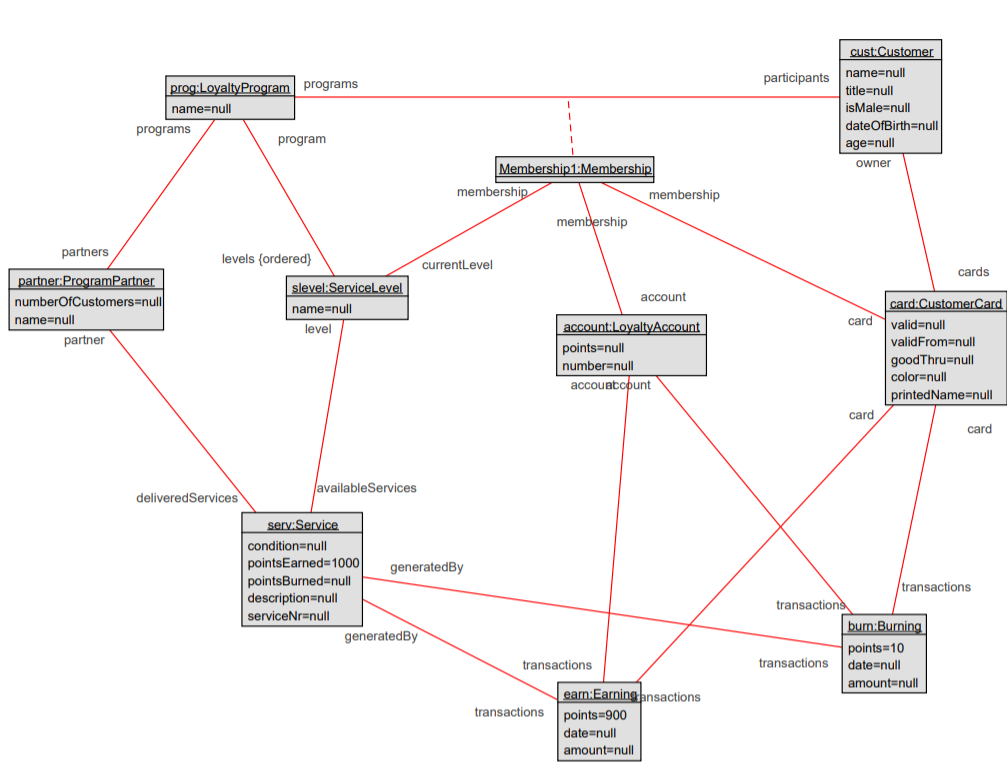
\includegraphics[width=\linewidth]{Q2obj.png}
		\caption{Royalty and Loyalty Object Diagram}
		\label{fig:q2obj}
	\end{figure}
	
	\noindent
	With Figure \ref{fig:q2obj} as the state of the system, we ran check on the use command line. Note that serv (of type Service) has pointsEarned = 1000 and earn (of type Earning) has points = 900. This state should not violate any constraint. It said that we were not violating any constraints, as shown in Figure \ref{fig:q2cmd}.
	
	\begin{figure}[h]
		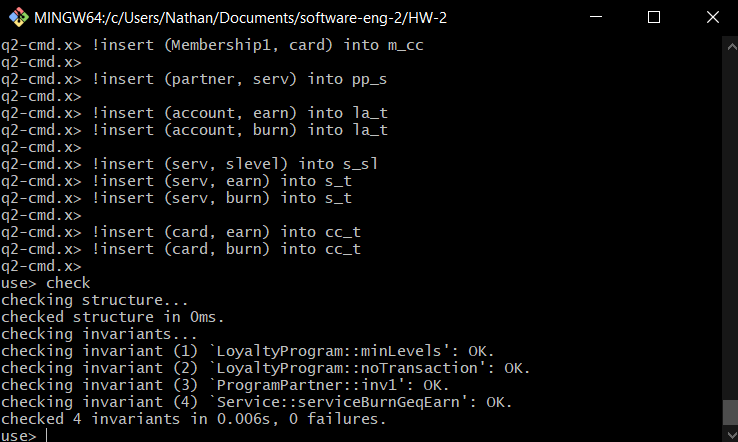
\includegraphics[width=\linewidth]{Q2cmd.png}
		\caption{Checking constraings on Royalty and Loyalty Model}
		\label{fig:q2cmd}
	\end{figure}
	
	\newpage
	\noindent
	Figure \ref{fig:q2cmd} shows that our the state did not violate the invariants.
	\newpage

\section*{Question 3}

The UML class model was given in the assignment sheet, so we only provided our .use file that produces an identical class model. This is shown below.

\begin{Verbatim}
model work

--person class
class Person
attributes
	name:String
	age:Integer
	salary:Real
operations
	raiseSalary(amount:Real):Real
end

--company class
class Company
attributes
	name:String
	location:String
operations
	hire(p:Person)
		begin
		end
	fire(p:Person)
		begin
		end
end

--associations

--association between Person and Company
association P_C between
	Person [*] role employee
	Company [0..1] role employer
end

--constraints

constraints

context Company::hire(p:Person)
	pre hirePre1: p.isDefined()
	post hirePost1: employee->includes(p)

context Company::fire(p : Person)
	pre  firePre:  employee->includes(p)
	post firePost: employee->excludes(p)

context Person::raiseSalary(amount : Real) : Real
	post raiseSalaryPost:
		salary = salary@pre+amount
\end{Verbatim}
	We found these pre and post conditions in the documentation on the following website: \newline
	http://useocl.sourceforge.net/w/index.php/Validate\_pre-\_and\_postconditions \\\\
	In Figures \ref{fig:hirefire} and \ref{fig:raisesal}, we show tests for the pre/post conditions on each of the methods decorated with OCL.
	\begin{figure}[h]
		\centering
		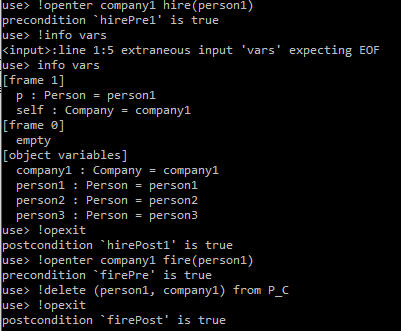
\includegraphics[width=.5\linewidth]{soil1.PNG}
		\caption{Hire and Fire Testing}
		\label{fig:hirefire}
	\end{figure}
	
	\begin{figure}[h]
		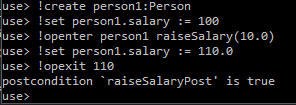
\includegraphics[width=\linewidth]{soil2.PNG}
		\caption{raiseSalary Testing}
		\label{fig:raisesal}
	\end{figure}

\end{document}